\documentclass[oneside,12pt]{DISCSthesis}
\usepackage{graphicx}
\usepackage{longtable}
\usepackage{setspace}
\usepackage{soul}
% \usepackage{xcolor}
\usepackage{amsmath}
\usepackage{algpseudocode}
	\renewcommand{\algorithmiccomment}[1]{\hskip0em$\triangleright$ \emph{#1}}
	\renewcommand{\algorithmicrequire}{\hspace*{6pt}\textbf{Input:}}
	\renewcommand{\algorithmicensure}{\hspace*{6pt}\textbf{Output:}}

\usepackage{moreverb}

%\documentclass{article}
\begin{document}
	\ThesisAuthor{\textbf{Maria Clara Isabel D. Sia}}
	\ThesisTitle{\textbf{\boldmath Improving An Exact Solution to the ($l$, $d$)-Planted Motif Problem}}
	\ThesisArea{Computer Science}
	\ThesisDefenseYear{2015}
	\DefenseDate{23 October 2015} % \ThesisGrade{}

	\DepartmentHead{MARLENE M. DE LEON, Ph.D.}
	\SchoolHead{EVANGELINE P. BAUTISTA, Ph.D.}
	\ThesisAdviser{PROCESO L. FERNANDEZ, JR., Ph.D.}
	\FirstPanelMember{ANDREI D. CORONEL, Ph.D.}
	\SecondPanelMember{JULIETA Q. NABOS}
	\ThirdPanelMember{JOSE ALFREDO A. DE VERA, Ph.D.}

	\ThesisStyle{MS}{FinalWithCorner}{-10pt}{15pt}

\FrontMatter % =======================================================

\begin{abstract}
	DNA motif finding is widely recognized as a difficult problem in computational biology and computer science. Because of the usual large search space involved, exact solutions typically require a significant amount of execution time before discovering a motif of length $l$ that occurs in an input set $\{S_{1} ,...,S_{n}\}$ of sequences, allowing for at most $d$ mismatches due to mutation. 

	This study implements a novel speedup technique for EMS-GT, an exact motif search algorithm which operates on a compact bit-based representation of the search space. Our novel technique takes advantage of distance-related patterns in this representation, in order to speed up the bulk bit-setting operations performed by the algorithm. A Java implementation shows the improved EMS-GT to be highly competitive against PMS8 and qPMS9, two current state-of-the-art exact algorithms. With the speedup technique, EMS-GT outperforms both competitors for challenging ($l,d$) instances (9,2), (11,3), (13,4) and (15,5) showing runtime reductions from qPMS9 of at least 76\%, 81\%, 77\% and 37\% respectively for these instances, while ranking second to qPMS9 for challenge instance (17,6).
	\end{abstract}

	\tableofcontents
	\listoffigures
	\listoftables

\MainMatter  % =======================================================

\chapter{INTRODUCTION}

\chapter{REVIEW OF RELATED LITERATURE}

\chapter{METHODOLOGY}


\chapter{RESULTS AND ANALYSIS}
	This section derives the distance-related patterns observed in an $l$-mer neighborhood (represented with a $4^l$-bit array) in EMS-GT. It then describes how a speedup technique for EMS-GT was developed based on these patterns. Finally, it compares EMS-GT performance with and without the speedup technique, and compares the performance of improved EMS-GT against state-of-the-art algorithms PMS8 and qPMS9.

	\section{\boldmath Block patterns in $l$-mer neighborhoods}
		We can represent the neighborhood of $l$-mer $x$ as an array $N_x$ of $4^{l}$ bit flags, set to 1 if the corresponding $l$-mer is a neighbor and 0 otherwise.\\
		\begin{equation}
			N_{x}[\ x'\ ] = \left\{
			\begin{array}{rl}
				1 & \text{if } d_H(x,x') \leq d,\\
				0 & \text{otherwise.}
			\end{array} \right.
			\text{ for any $l$-mer }x'.
			\end{equation}\\
		\noindent We can divide our $l$-mer $x$ into its {\bf\boldmath prefix $y$} (the first $l-k$ characters) and its {\bf\boldmath $k$-suffix $z$} (the last $k$ characters). We use the notation $x$ = $yz$.
		\begin{center}
			Ex. For $k$ = 5,\ \ $x$ = \texttt{acgtacgtacgt} $\rightarrow$ \ \ $y$ = \texttt{acgtacg} and $z$ = \texttt{tacgt}.
			\end{center}
		\noindent If we partition $N_x$ into blocks of $4^k$ bits each, for some $k < l$, the $4^k$ $l$-mers represented in each block will all start with the same {\bf block prefix} and all have different $k$-suffixes.	This is because $N_x$ represents $l$-mers in alphabetical order.
		\begin{center} 
			Ex. Blocks in $N_x$ for $x$ = \texttt{acgtacgtacgt},\ \ $k$ = 5:
			\ \ \ \ \ \ \ \ \ \ \ \ \ \ \ \ \ \ \ \ \ \ \ \ \ \ \ \ \ \ \\
			\footnotesize
			Block 0:\ \ \ \ \ \ \ \ \ \ \ \ \ \ \ \ \ \ bit flags for \texttt{{aaaaaaa}\ul{aaaaa} - {aaaaaaa}\ul{ttttt}}\\
			Block 1:\ \ \ \ \ \ \ \ \ \ \ \ \ \ \ \ \ \ bit flags for \texttt{{aaaaaac}\ul{aaaaa} - {aaaaaac}\ul{ttttt}}\\...\\
			Block 1,734:      \ \ \ \ \ \ \ \ \ \ \ \ \ bit flags for \texttt{{acgtacg}\ul{aaaaa} - {acgtacg}\ul{ttttt}}\\...\\
			Block 16,833:           \ \ \ \ \ \ \ \ \ \ bit flags for \texttt{{ttttttg}\ul{aaaaa} - {ttttttg}\ul{ttttt}}\\
			Block 16,834:           \ \ \ \ \ \ \ \ \ \ bit flags for \texttt{{ttttttt}\ul{aaaaa} - {ttttttt}\ul{ttttt}}\\\ \\
			\end{center}
		\noindent Each such block in $N_x$ will also conform to one of ($k+2$) bit patterns.\vspace*{4mm}

		\begin{figure}[h]\label{fig:block_patterns}
			\footnotesize\centering
			\begin{minipage}{.135\textwidth}\centering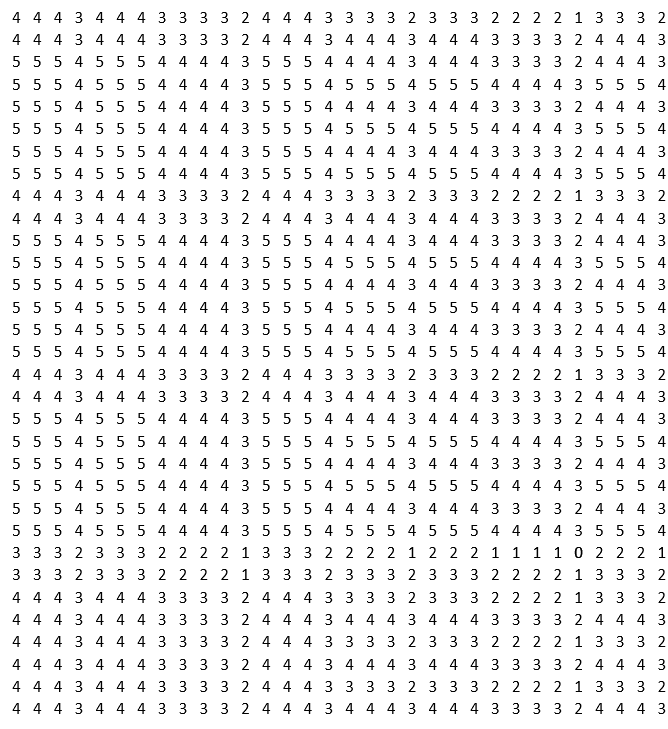
\includegraphics[width=0.95\textwidth]{img/-1}\\ Pattern -1 \end{minipage} 
			\begin{minipage}{.135\textwidth}\centering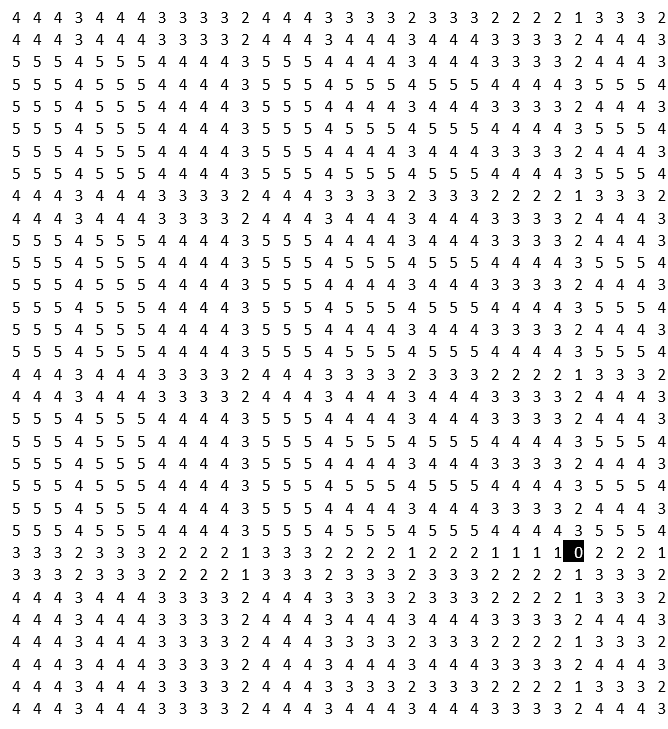
\includegraphics[width=0.95\textwidth]{img/0}\\ Pattern 0 \end{minipage} 
			\begin{minipage}{.135\textwidth}\centering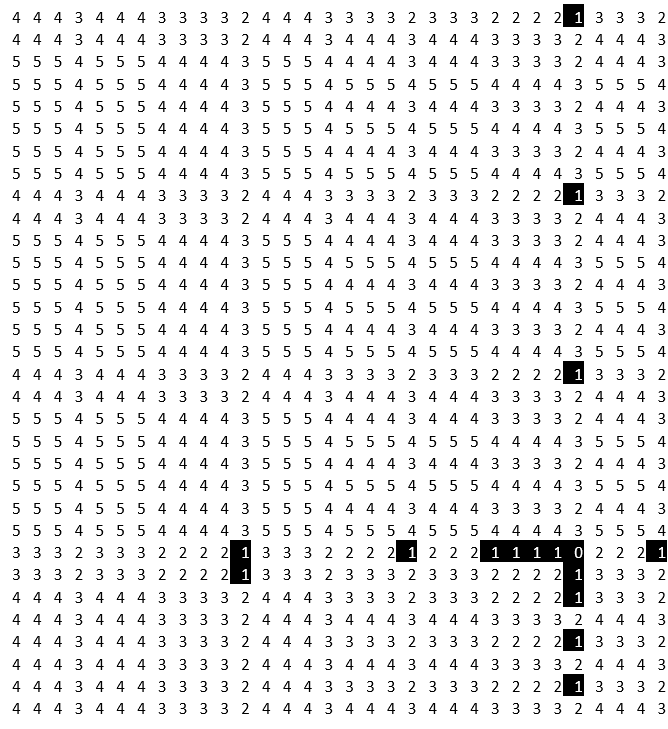
\includegraphics[width=0.95\textwidth]{img/1}\\ Pattern 1 \end{minipage}
			\begin{minipage}{.135\textwidth}\centering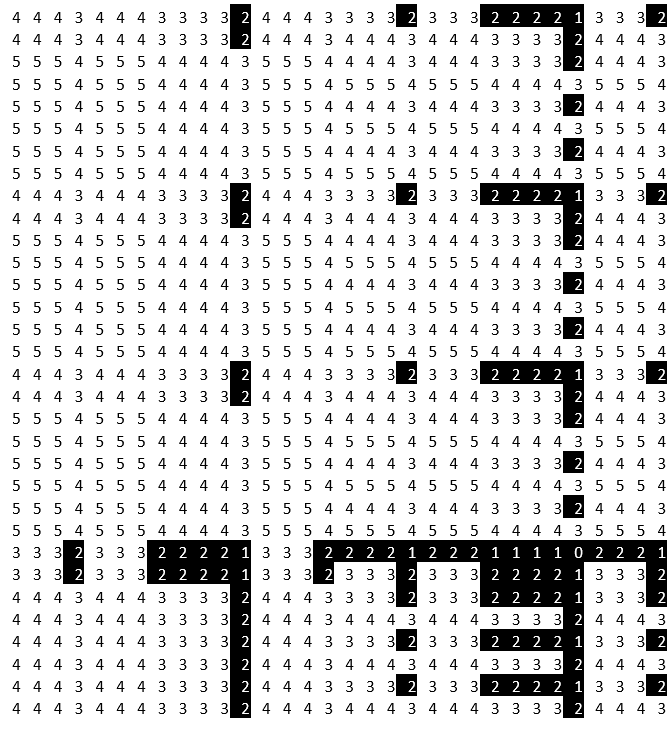
\includegraphics[width=0.95\textwidth]{img/2}\\ Pattern 2 \end{minipage}
			\begin{minipage}{.135\textwidth}\centering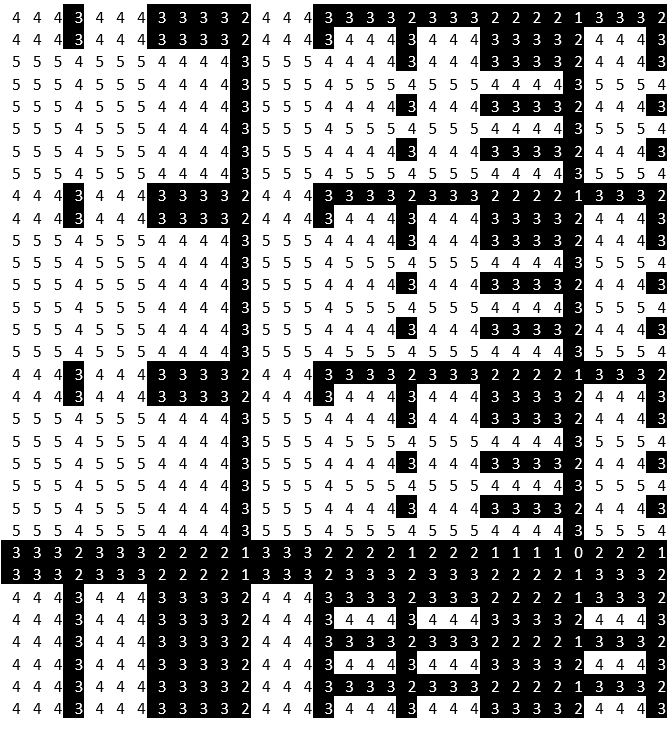
\includegraphics[width=0.95\textwidth]{img/3}\\ Pattern 3 \end{minipage}
			\begin{minipage}{.135\textwidth}\centering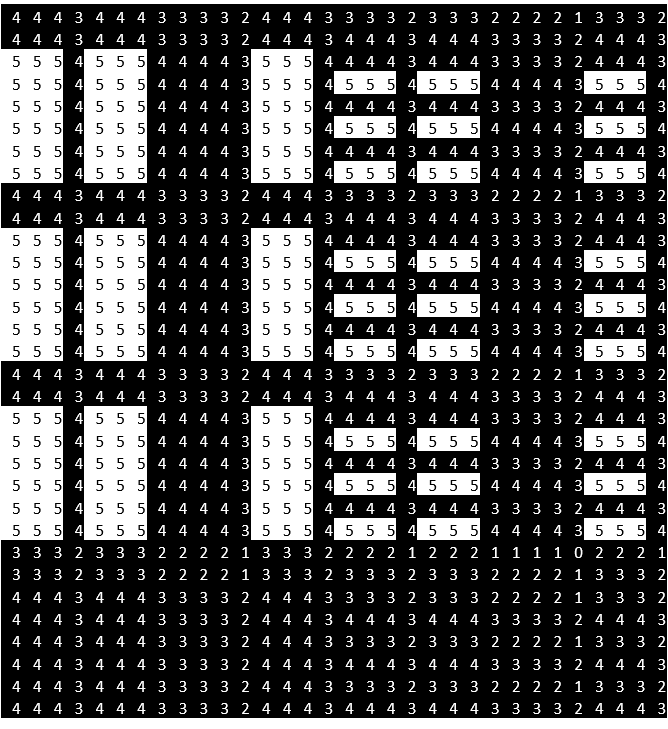
\includegraphics[width=0.95\textwidth]{img/4}\\ Pattern 4 \end{minipage}
			\begin{minipage}{.135\textwidth}\centering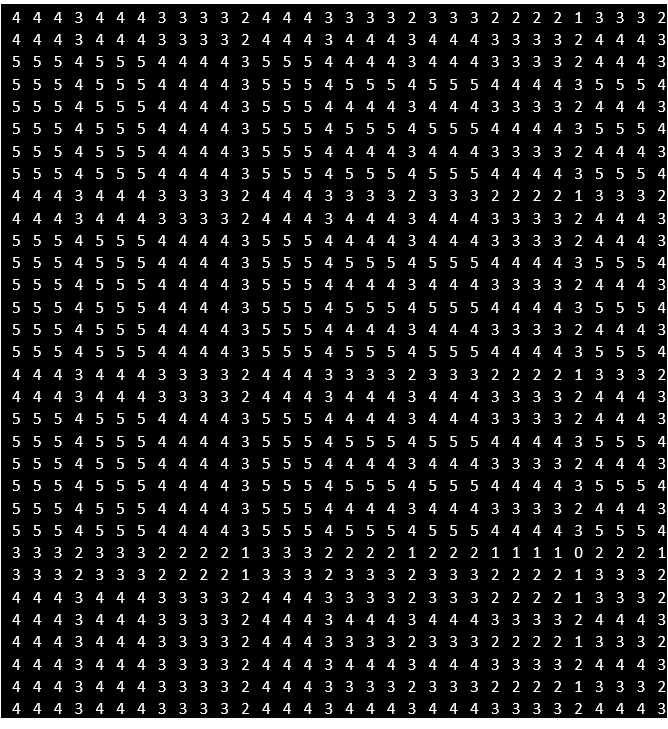
\includegraphics[width=0.95\textwidth]{img/5}\\ Pattern 5 \end{minipage}
			\newline\newline
			\caption{Bit patterns followed by blocks in the bit-array representation of $N(\texttt{acgtacgtacgt}, 5)$. 
			Black signifies a bit set to 1.}
			\end{figure}

		\noindent If we can derive these pattterns, we will be able to build $N_x$ in blocks, instead of setting bits one by one as EMS-GT currently does. The next section uses the additive property of Hamming distances to derive the bit patterns in $N_x$.
		\newpage

	\section{Derivation of patterns based on Hamming distances}
		\noindent Since Hamming distances count mismatches in corresponding characters, the distance between $x = yz$ and another $l$-mer $x' = y'z'$ is the sum of the mismatches between their prefixes and the mismatches between their $k$-suffixes, or:\vspace*{-4mm} 
		\begin{equation} d_H(x,x') = d_H(y,y') + d_H(z,z')\vspace*{-4mm}\end{equation}
		Given Equations (4.1) and (4.2), we can redefine $N_x$ as:\vspace*{-4mm}
		\begin{equation}
			N_{x}[\ x'\ ] = \left\{
			\begin{array}{rl}
				1 & \text{if } d_H(y,y') + d_H(z,z') \leq d,\\
				0 & \text{otherwise.}
			\end{array} \right.
			\text{ for }x' = y'z'.\vspace*{-4mm}	
			\end{equation}
		Intuitively, if $x$ and $x'$ are neighbors, and there are {\bf\boldmath $d_H(y,y')$  prefix mismatches} between them, we can  allow {\bf\boldmath $d_H(z,z') \leq d - d_H(y,y')$ $k$-suffix mismatches} for $x$ and $x'$ to have $d$ or fewer total mismatches. Table 4.\ref{tbl:cases_prefix_suffix} shows the ($k+2$) cases for distributing $d$ allowable mismatches between prefix and $k$-suffix. \vspace*{3mm}

		\begin{table}[h] \label{tbl:cases_prefix_suffix}
			\centering\renewcommand{\arraystretch}{1.3}
			\begin{tabular}{|l|r|l|}
			\hline
			\bfseries & \bfseries prefix mismatches & \bfseries\boldmath $k$-suffix mismatches \\
			\hline
			Case -1 &		more than $d$ 	& --\\
			Case  0 & 		$d$ 			& 0 \\
			Case  1 & 		$d$ - 1 		& 0, 1 \\
			Case  2 & 		$d$ - 2 		& 0, 1, 2 \\
			... & ...& ...\\
			Case  $k$-1 & 	$d$ - ($k$-1) 	& 0, 1, 2, ..., ($k$-1) \\
			Case  $k$ & 	$d-k$ or less 	& 0, 1, 2, ..., ($k$-1), $k$ \\
			\hline
			\end{tabular}
			\caption{Allowable suffix mismatches, for a fixed number of prefix mismatches, between $d$-neighbors.}
			\end{table}
		
		\newpage
		\noindent The ($k+2$) cases shown in Table 4.\ref{tbl:cases_prefix_suffix} correspond to the ($k+2$) bit patterns followed by the blocks in $N_x$. The value of $d_H(y,y')$ determines which pattern applies to which block:

		\begin{figure}[h]\label{fig:cases_block_patterns}
			\footnotesize
			\begin{minipage}{.33\textwidth}\centering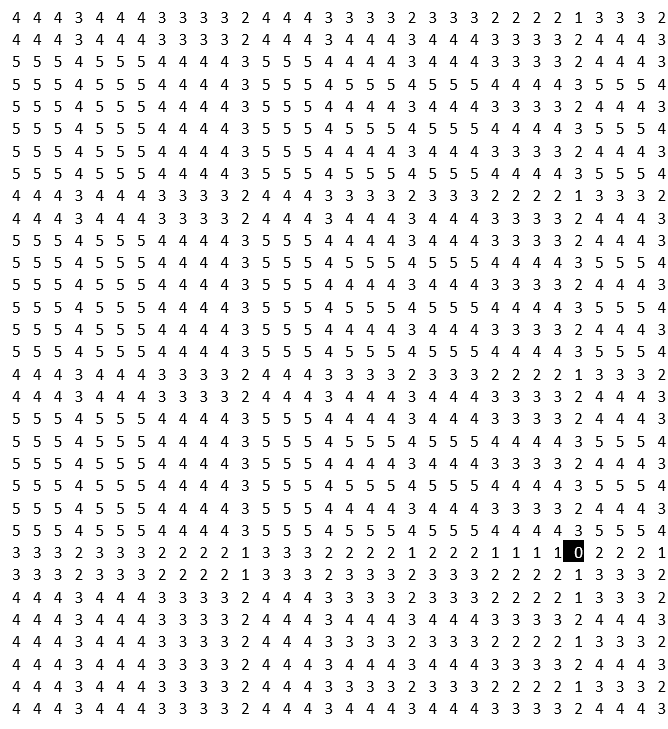
\includegraphics[width=0.95\textwidth]{img/0}\\ $d_H(y,y') = d$ \end{minipage} 
			\begin{minipage}{.33\textwidth}\centering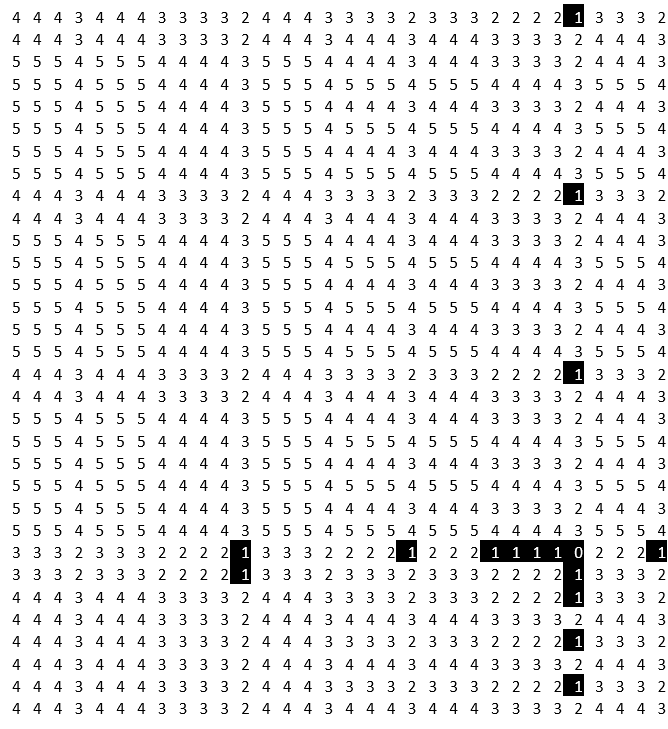
\includegraphics[width=0.95\textwidth]{img/1}\\ $d_H(y,y') = d-1$ \end{minipage}
			\begin{minipage}{.33\textwidth}\centering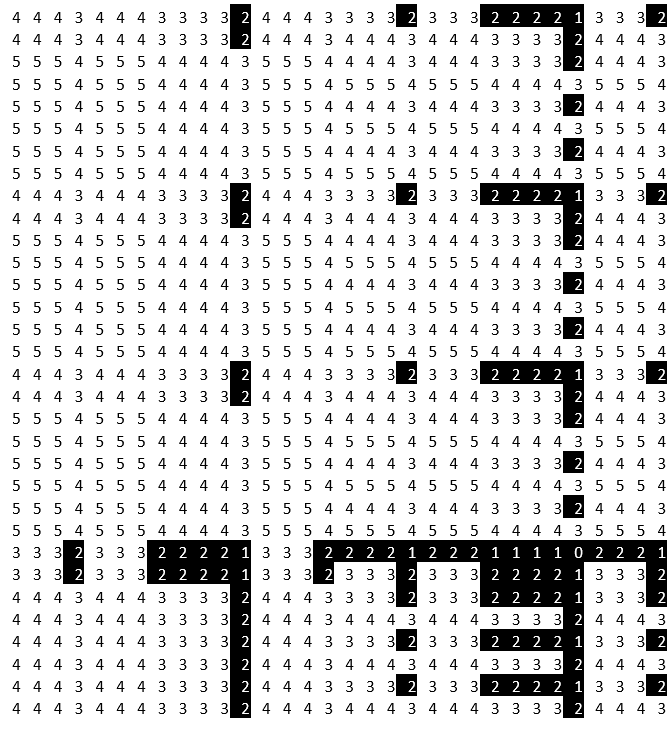
\includegraphics[width=0.95\textwidth]{img/2}\\ $d_H(y,y') = d-2$ \end{minipage}
			\\\ \\\ \\\ \\
			\begin{minipage}{.33\textwidth}\centering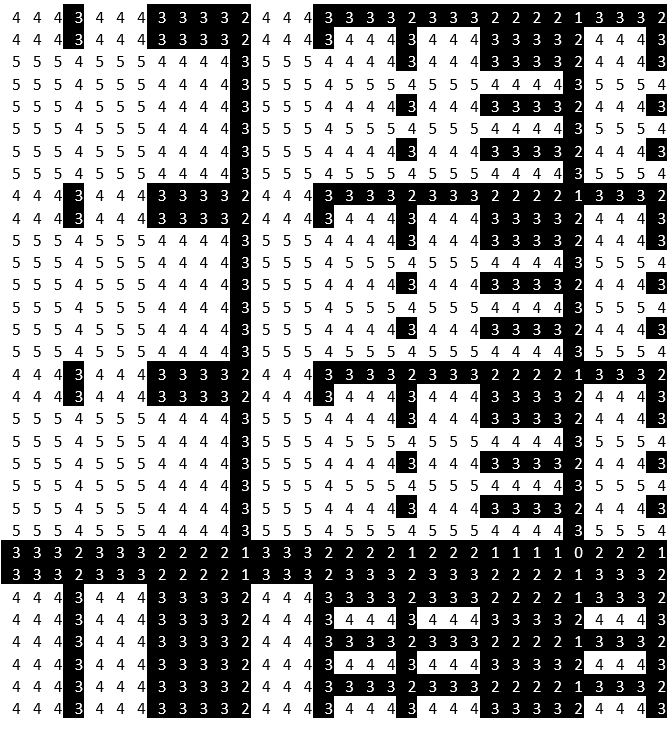
\includegraphics[width=0.95\textwidth]{img/3}\\ $d_H(y,y') = d-3$ \end{minipage}
			\begin{minipage}{.33\textwidth}\centering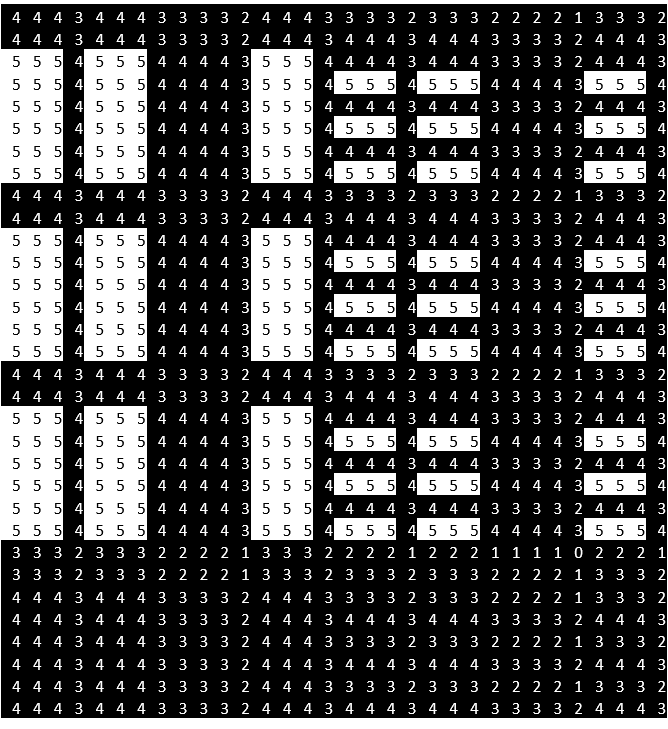
\includegraphics[width=0.95\textwidth]{img/4}\\ $d_H(y,y') = d-4$ \end{minipage}
			\begin{minipage}{.33\textwidth}\centering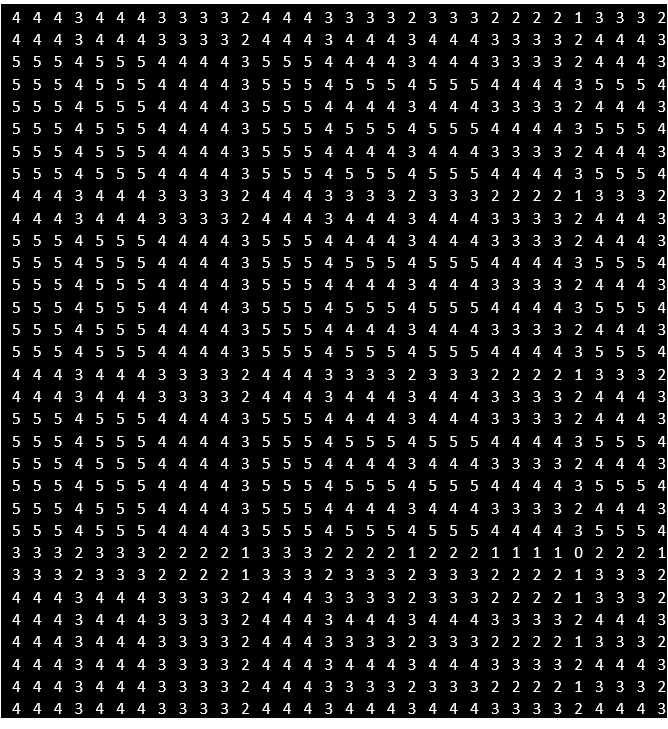
\includegraphics[width=0.95\textwidth]{img/5}\\ $d_H(y,y')\leq d-5$ \end{minipage}
			\newline\newline
			\caption{Correspondence between the value of $d_H(y,y')$ and bit patterns for $N(\texttt{acgtacgtacgt}, 5)$. 
			Black signifies a bit set to 1.}
			\end{figure}

		\noindent Note that when $d_H(y,y') > d$, the number of prefix mismatches already exceeds the limit for neighbors, hence no bits in the block are set (see Pattern -1, Fig 4.\ref{fig:block_patterns}).

		\newpage
		%%%%%%% To-do: explain here the suffix distribution to generate patterns etc.
		\noindent The specific configuration of bits in each of the patterns is according to the distribution of Hamming distances from $x$'s $k$-suffix $z$, to all possible $k$-suffixes $z'$. We know that 

		\begin{figure}[h] \label{fig:D_tacgt}
			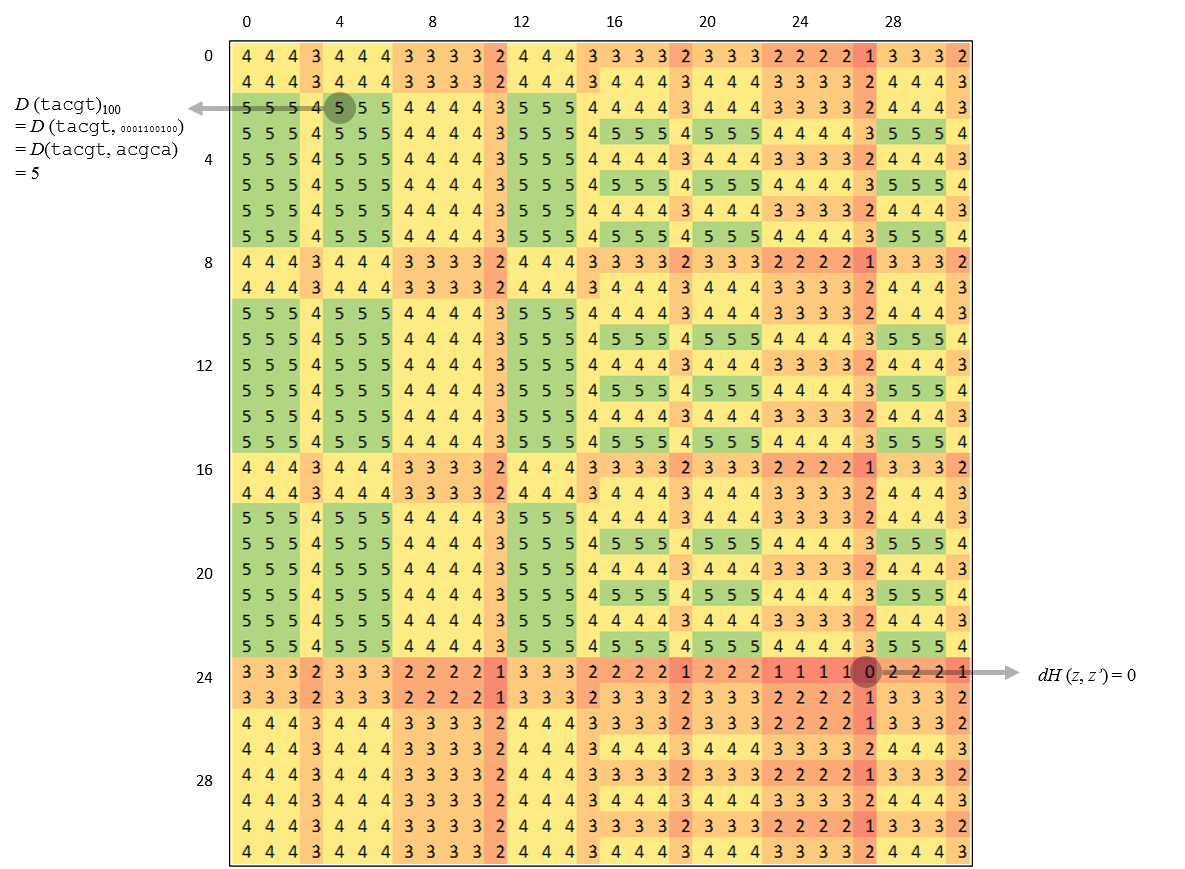
\includegraphics[width=6.0in]{img/D(tacgt)_marked_2}
			\caption{Distance distribution from \texttt{tacgt} to all $4^{5} = 32 \times 32$ $k$-suffixes, $k$=5.}
			\end{figure}

		%%%%%%% To-do: mathematical definition of Pattern i.e. P[ j ] { 1 if d_H(z,z') \leq j, 0 otherwise

	\section{Pattern-based EMS-GT speedup technique}
		\begin{enumerate}
			\item Step 1
			\item Step 2
			\end{enumerate}

	\section{Performance improvement in EMS-GT}

	\section{Performance comparison to PMS8 and qPMS9}


\chapter{CONCLUSIONS}
	In line with our research objectives, we make the following conclusions:

	\begin{enumerate}
	\item Our novel speedup technique takes advantage of the distance-related block patterns observed in the search space. Initially EMS-GT generates, and sets the bit for, each individual neighbor of an $l$-mer $x$. However, our speedup technique allows EMS-GT to set these bits in blocks of $4^k$ bits each, using pre-generated bit patterns; we find the ideal value of $k$ to be 5.
	\item The speedup technique improves EMS-GT's performance on challenging ($l$,$d$) instances (11,3), (13,4), (15,5) and (17,6), with runtime reductions of at least 6.7\%, 47.5\%, 38.1\% and 43.0\% respectively; however, on challenge instance (9,2), overhead increases EMS-GT's runtime from 0.06 s initially to 0.11 s with the speedup technique.
	\item The speedup technique allows EMS-GT to outperform the current best algorithm, qPMS9, on challenging ($l$,$d$) instances (9,2), (11,3), (13,4) and (15,5) with runtime reductions of at least 76\%, 81\%, 77\% and 37\% respectively for these instances, while ranking second to qPMS9's runtime on challenge instance (17,6).
	\end{enumerate}

	\noindent Directions for further research on improving EMS-GT include:

	\begin{enumerate}
	\item Refining the bit-based search space representation (i.e. with compression techniques) to be able to represent the motif search space for $l > 17$;
	\item Creating a multiprocessor version of EMS-GT to solve the planted motif problem faster, in parallel, for larger values of ($l$, $d$); and
	\item Delegating the bit-masking speedup technique and other bulk bit operations to the graphics card, as explored in \cite{dasari2010efficient}, for faster performance.
	\end{enumerate}


\BackMatter  % =======================================================
	\bibliographystyle{plain}
	\bibliography{sources}

\appendix{Source code for EMS-GT, with speedup technique}


\end{document}